\documentclass[10pt,a4,oneside]{article}
\usepackage{a4wide}
\usepackage{graphicx}
\parindent=0pt

\begin{document}
\begin{titlepage}
\begin{center}

\vfill
\textbf{\huge Milestone 4 Report}\\ \textit{} \\ \textit{} 
\textit{for} \\ \textit{} \\ \textit{} 
\textbf{\huge Group 1}\\ \textit{} \\ \textit{}
\vfill
\textbf{Alex Egan \\ Filimoni Lutunaika \\ George Sainsbury \\ Xiaodong Cui}
\end{center}
\end{titlepage}

\newpage

\paragraph{}

\tableofcontents

\[----\]

\newpage

\section{Introduction}

\paragraph{}
Group 1 was assigned Tickets 75, 131, 174 and 186 for Milestone 4. Ticket 75 implemented listing by either name OR (with a slight modification) size. Ticket 131 made it configurable for either use file bytes or real disk usage in all web applications. Ticket 174 allowed earth to release a gem. Ticket 186 implemented remove feature for earth.

\section{Resources}

\paragraph{}
Group 1 comprised an equal split of 2 Bachelor of Engineering (Software Engineering)
 students and 2 Master of Software of Engineering students. This provided the Group with
  approximately 72 hours of available development time per week, this estimate is based on 
  the 6 hours per week coursework commitment that the school expects from each BESE student 
  and 30 hours per week for each MSE students.

\section{Task Allocation}

\paragraph{}
For Milestone 4, the distribution tasks amongst the members were based on among other 
things the hours that each member was expected to commit to the project. As a result, the tasks were distributed as the following.

\begin{itemize}
 \item Alex:   Ticket 75 sort by name or size.
 \item George: Ticket 174 creating the Earth Gem.
 \item Fili:   Ticket 186 remove feature of Earth Daemon and also in charge of managing the repository for Subgroup 1. This includes ensuring that the Milestone 4 solutions undergo integration testing before being committed onto the Subgroup 1 repository.
 \item Cui:    Ticket 131 use real disk usage instead of byte size and also in charge of writing documents for group 1.
\end{itemize}

\newpage

\section{Resource Allocation}

\paragraph{}
The table below shows the planned time and actual time for each group member spent on the assigned tasks.

\begin{table}[ht!]
\begin{tabular}{|p{5cm}|p{1.5cm}|p{1.5cm}|} 
\hline
 & & \\
Tasks & Planned Time & Actual Time\\
 & & \\
\hline
 & & \\
Alex (Ticket 75) & 10hrs & 17hrs\\
 & & \\
\hline
 & & \\
George (Ticket 174) & 10hrs & 6hrs\\
 & & \\
\hline
 & & \\
Fili (Ticket 186) & 81hrs & 87hrs\\
 & & \\
\hline
 & & \\
Cui (Ticket 131) & 73hrs & 70hrs\\
 & & \\
\hline
 & & \\
Total & 175hrs & 180hrs\\
 & & \\
\hline
\end{tabular}
\end{table}

For detailed resource allocation, please refer to individual report.
\section{Activity Summary}

\paragraph{}
The tasks assigned to group 1 have been successfully completed, and each group member seemed to have successfully made a serious attempt in their respective tasks. However since every group member was working on different ticket, it was no clear collaborative development opportunities within the group; and the resources were only allocated to group members to finish their individual tasks, so it was almost impossible to manage the group resources as a whole. The resources were allocated based on individually estimated efforts on their tasks, and that may different from person to person. Based on the Group's Milestone 4 achievements, it could be safely assumed that the distribution of tasks was at least fair. Ticket 174, 131 and 186 were completed, but ticket 75 was not completed, and that is because BESE students had limited time (6-8 hours per week) to do their tasks, and the remaining tasks would be expected to be completed in next milestone. 

\section{Progress Summary}

\paragraph{}
The progress summary for group1 is listed below:

\begin{itemize}
 \item Alex: Ticket 75 incomplete.
 \item George: Ticket 174 completed
 \item Fili: Ticket 186 completed.
 \item Cui: Ticket 131 completed.
\end{itemize}

\newpage

\section{Conclusions}

\paragraph{}
\noindent Group 1 managed to complete tickets 174, 186 and 131 and the relevant codes could be obtained from the GitHub repository. Ticket 75 is expected to be completed in next milestone.

\newpage

\section{Individual Milestone 4 Report - Alex Egan}

\subsection*{Task Description}
The task assigned to me was Ticket 75. This deals with dynamic sorting of the output in the Navigation and All Files tabs in the Earth application. The goal was to be able to click on a column heading, such as Name or Size, and have the file listing be sorted by the appropriate criterion.

\subsection*{Progress Summary}
\label{prog-sum}
The ticket was not completed as required. Investigations into the changes to be made revealed bugs in the current implementation of the pagination on the All Files view and the sorting of the columns. The All Files view has the dynamic sorting that the ticket requires implemented but it does not work when there is only one page of files to list. The sorting also takes two parameters so that it can sort by name and then by file size, for example. There is an arrow icon that indicates ascending or descending sort order by pointing up or down. The default sort state causes this icon to not show initially and this is another issue that needs to be addressed.\\
\\
The plan was to use the current code as much as possible and to use the All Files implementation as the basis for the Navigation tab to ensure visual and code consistency. I tried to fix the bugs but was unsuccessful in my attempts. Once these are fixed it will be easier to add the necessary changes for the Navigation tab.

\subsection*{Resource Allocation}
The estimate as in the plan is below.\\
\\
\textbf{Subtasks:}
\begin{enumerate}
	\item Design and code the dynamic sorting of record listing. (7 hrs)
	\item Test and integrate solution to the Subgroup 1 codebase. (2 hrs)
	\item Update the Earth Trac system. (1 hr)
\end{enumerate}
\textbf{Total Time Estimate:} 10 hrs

\subsection*{Resource Use}
See the Time Log in Section \ref{time-log} for detailed time spent on the tasks.\\
\\
The task was not completed on schedule. Once work began on this task, it became apparent that the planned approach was not going to work. The planned subtasks should have been more refined. The largest issue was understanding the existing code and how it works. Trying understand Haml proved more difficult than expected. The discovery of the bugs mentioned in Section \ref{prog-sum} was unexpected.\\
\\
To improve progress in the next sprint, working with someone who has a better knowledge of Haml, perhaps through pair programming, will assist in finding the issues that need to be resolved and help me improve my understanding of the markup language. This will assist in making progress on other tasks in the future as well.

\subsection*{Time Log}
\label{time-log}
%week 1
\subsection*{Semester 2, Week 1}
\subsubsection*{Monday Jul 28, 2008}
1300 - 1500 hrs\\
Attended main group meeting and discussed planned tasks for Milestone 4.\\
\\
\textbf{Daily Total} 2 hrs\\

\subsubsection*{Thursday Jul 31, 2008}
1800 - 2000 hrs\\
Looked through Earth code to find the appropriate files to be modified for completion of the task. Began trying to figure out how the code works.\\
\\
\textbf{Daily Total} 2 hrs\\
\\
\textbf{Weekly Total:} 4 hrs

%week 2
\subsection*{Semester 2, Week 2}
\subsubsection*{Monday Aug 4, 2008}
1300 - 1400 hrs\\
Attended main group meeting and discussed progress.\\
\\
\textbf{Daily Total:} 1 hrs

\subsubsection*{Wednesday Aug 6, 2008}
1400 - 1500 hrs\\
Attended Group 1 subgroup meeting with Dr Li.\\
\\
1900 - 2000 hrs\\
Discovered that my installation of Earth wasn't working when I tried to test some changes. Tried to remedy it unsuccessfully.\\
\\
\textbf{Daily Total:} 2 hrs\\

\subsubsection*{Thursday Aug 7, 2008}
1700 - 1900 hrs\\
Got Earth working again. Coding.\\
\\
\textbf{Daily Total:} 2 hrs\\
\\
\textbf{Weekly Total:} 5 hrs

%week 3
\subsection*{Semester 2, Week 3}
\subsubsection*{Monday Aug 11, 2008}
1300 - 1400 hrs\\
Group Meeting at Software Engineering Meeting Room\\
\\
2000 - 2300 hrs\\
Coding and discovered bugs in All Files tab.\\
\\
\textbf{Daily Total} 4 hrs\\

\subsubsection*{Wednesday Aug 11, 2008}
2000 - 2200 hrs\\
Coding.\\
\\
\textbf{Daily Total} 2 hrs\\

\subsubsection*{Friday Aug 15, 2008}
0300 - 0400 hrs\\
Presentation preparation.\\
\\
1400 - 1500 hrs\\
Attended Milestone 4 presentation.\\
\\
\textbf{Daily Total:} 2 hrs\\
\\
\textbf{Weekly Total:} 8 hrs\\
\\
\textbf{Sprint Total:} 17 hrs%%%%

\newpage
\section{Individual Milestone 4 Report - Xiaodong Cui}

\paragraph{} By Xiaodong Cui (1149546)


\subsection*{Introduction}

\paragraph{}
I was assgined tasks to do ticket 131 and prepare documentation for group 1 at the beginning of milestone 4. Ticket 131 is about using real disk usage instead of byte size for all web applications. At present, it is configurable for users to decide whether use file bytes or real disk size by just setting in earth-webapp.yml file.

\subsection*{Task Description}

\paragraph{}
We are now gathering disk space usage (calculated as number of occupied 512-byte blocks) along with the size of each file, This is a better/more precise metric for determining where disk space is used, which probably is Earth's main purpose at this time. Therefore, the GUI should use this value instead in all situations. One solution had been implemented during milestone 3, but it was fragmented and could not be configurable by users. During milestone 4 I implemented a solution that could be configurable by users. The main task was broken down into four subtasks, and the resources were allocated to those subtasks. The documentation part includes setting meeting agendas, organising progress update meetings and writing plans and reports for group 1.

\subsection*{Resource Management}

\paragraph{}
As a master student, basically I have approximately 30 hours per week working on the project, totally about 90 hours for milestone 4.
\begin{itemize}
 \item Ticket 131 - Use real disk usage instead of byte size throughout the web application.
	\begin{itemize}
	\item Sub-task 1: Investigate potential solutions:
			\begin{itemize}
			\item Description: I spent about 16 hours to understand the relative web structure of earth, tried to find better solutions. Another 4-6 hours were spent on investigate the feasibility of solutions.
			\item Planned Time: 24 hours
			\item Actural Time: 21 hours (week 1 31/07/08-03/08/08)
			\end{itemize}
		\item Sub-task 2: Design solution
			\begin{itemize}
			\item Description: The previous solution uses disk size only, the current solution make it configurable for users to decide whether use disk size or file size for web application. Based on Investigation part, I designed the implementation structure for the solution
			\item Planned Time: 25 hours
			\item Actural Time: 19 hours (week 2 03/08/08-07/08/08)
			\end{itemize}
		\item Sub-task 3: Code solution
			\begin{itemize}
			\item Description: The actually coding for the solution. Changed and added some code to get the solution implemented. Refer to Appendix A to check files have been modified.
			\item Planned Time: 15 hours
			\item Actural Time: 17 hours (week 2 07/08/08- week 3 11/08/08)
			\end{itemize}
 		\item Sub-task 4: Test solution
			\begin{itemize}
			\item Description: This is to test the solution to see if the requirements specified in the Ticket description have been met, and to correct errors from test results.
			\item Planned Time: 6 hours
			\item Actural Time: 11 hours (week 3 11/08/08-13/08/08)
			\end{itemize}
		\item Sub-task 5: Integrate solution to the Subgroup 1 codebase
			\begin{itemize}
			\item Description: The new solution has been integrated to Subgroup 1 codebase.
			\item Planned Time: 2 hours
			\item Actural Time: 2 hours (week 3 13/08/08)
			\end{itemize}
		\item Sub-task 6: Update the Earth Trac system
			\begin{itemize}
			\item Description: Earth Trac system must be updated with the solution, but currently the system is down, I may update it later.
			\item Planned Time: 1 hours
			\item Actural Time: 0 hours
			\end{itemize}
		\item Total Planned Time: 73 hours
		\item Total Actual Time: 70 hours
		\end{itemize}
\item Documentation for group 1	
		\begin{itemize}
		\item This includes writing Agenda, minutes, report and plan for subgroup 1.
		\item Actual Time: 6 hours
		\end{itemize}
\end{itemize}

\subsection*{Implementation}

\paragraph{}
The solution was aimed to make it configurable by users to decide whether use file bytes or disk size in web application. A variable @size\_type was included in earth-webapp.yml for size configuration, and the value for this variable then was used as a flag to control what could be displayed on web pages. Also a new variable diskSize was added to Size.rb to represent the disk usage size. Based on this design, users can decide which size information they want to see on web pages, it is more flexible than just using real disk usage size.

\subsection*{Milestone 4 Summary}

\paragraph{}
During milestone 4, the main time was spent on investigation and design potential solutions. I spent more time than I initially expected, this is because I need to understand the structure on how earth to control what need to be displayed on web applications. Also I need to gether all relevant information on how to implement the solution using ruby on rails. Once the investigation and design parts finished, other parts were relatively easier to get implemented. I also felt that we did not have enough communication between group members, this is because each of us was working on different ticket, and tickets were not connected, so we had little chance to work together with others.

\subsection*{Conclusion}

\paragraph{}
The main task Ticket 131 was completed in milestone 4. However, there are may some other solution better than the current one, as I continue gaining experience on ruby and rails and earth project, I may find better solution for this ticket.

\section*{Appendix A - Modified Files}

\begin{itemize}
 \item Navigation:
	\begin{itemize}
 	\item size.rb
	\item application\_helper.rb
	\item server.rb
	\item directory.rb
	\item show.html.haml
	\end{itemize}
 \item All files
	\begin{itemize}
 	\item flat.html.haml
	\item browse\_controller.rb
	\end{itemize}
\item Radial views
	\begin{itemize}
 	\item graph\_helper.rb
	\item graph\_controller.rb
	\end{itemize}
\end{itemize}

\newpage

\section{Individual Milestone 4 Report - Filimoni Lutunaika}

\paragraph{} By Filimoni Lutunaika (1154924)

\subsection*{Introduction}

The Earth daemon operates by monitoring the size and file constituency of 
selected directories. This functionality requires the daemon to be able to 
add and remove monitored directories on-the-fly. The daemon can add 
directories to be monitored but the feature to remove or cease monitoring 
directories had yet to be implemented. The only way to remove directories 
was to access and directly manipulate the backend database.


\paragraph{}

\subsection*{Task Description}

Ticket 186 proposes the actual implementation of the remove directory 
feature and the relevant provisions already exists in the Earth daemon 
code. In fact, the daemon script recognises the remove option as a valid 
command but simply indicated that the feature is not functional. This 
existing deficiency provides the basis for investigating how this feature 
can be effectively integrated into the existing codebase.



\newpage

\subsection*{Implementation}

\paragraph{}
To help ensure that the implementation of the remove feature is consistent 
with the original vision of the Earth project developers, the investigative 
tasks focussed initially on identifying the existing implementation of the 
add feature. 


\paragraph{}
First, the following modifications were made to the Earth daemon code:


\begin{figure}[h!]
\begin{centering}
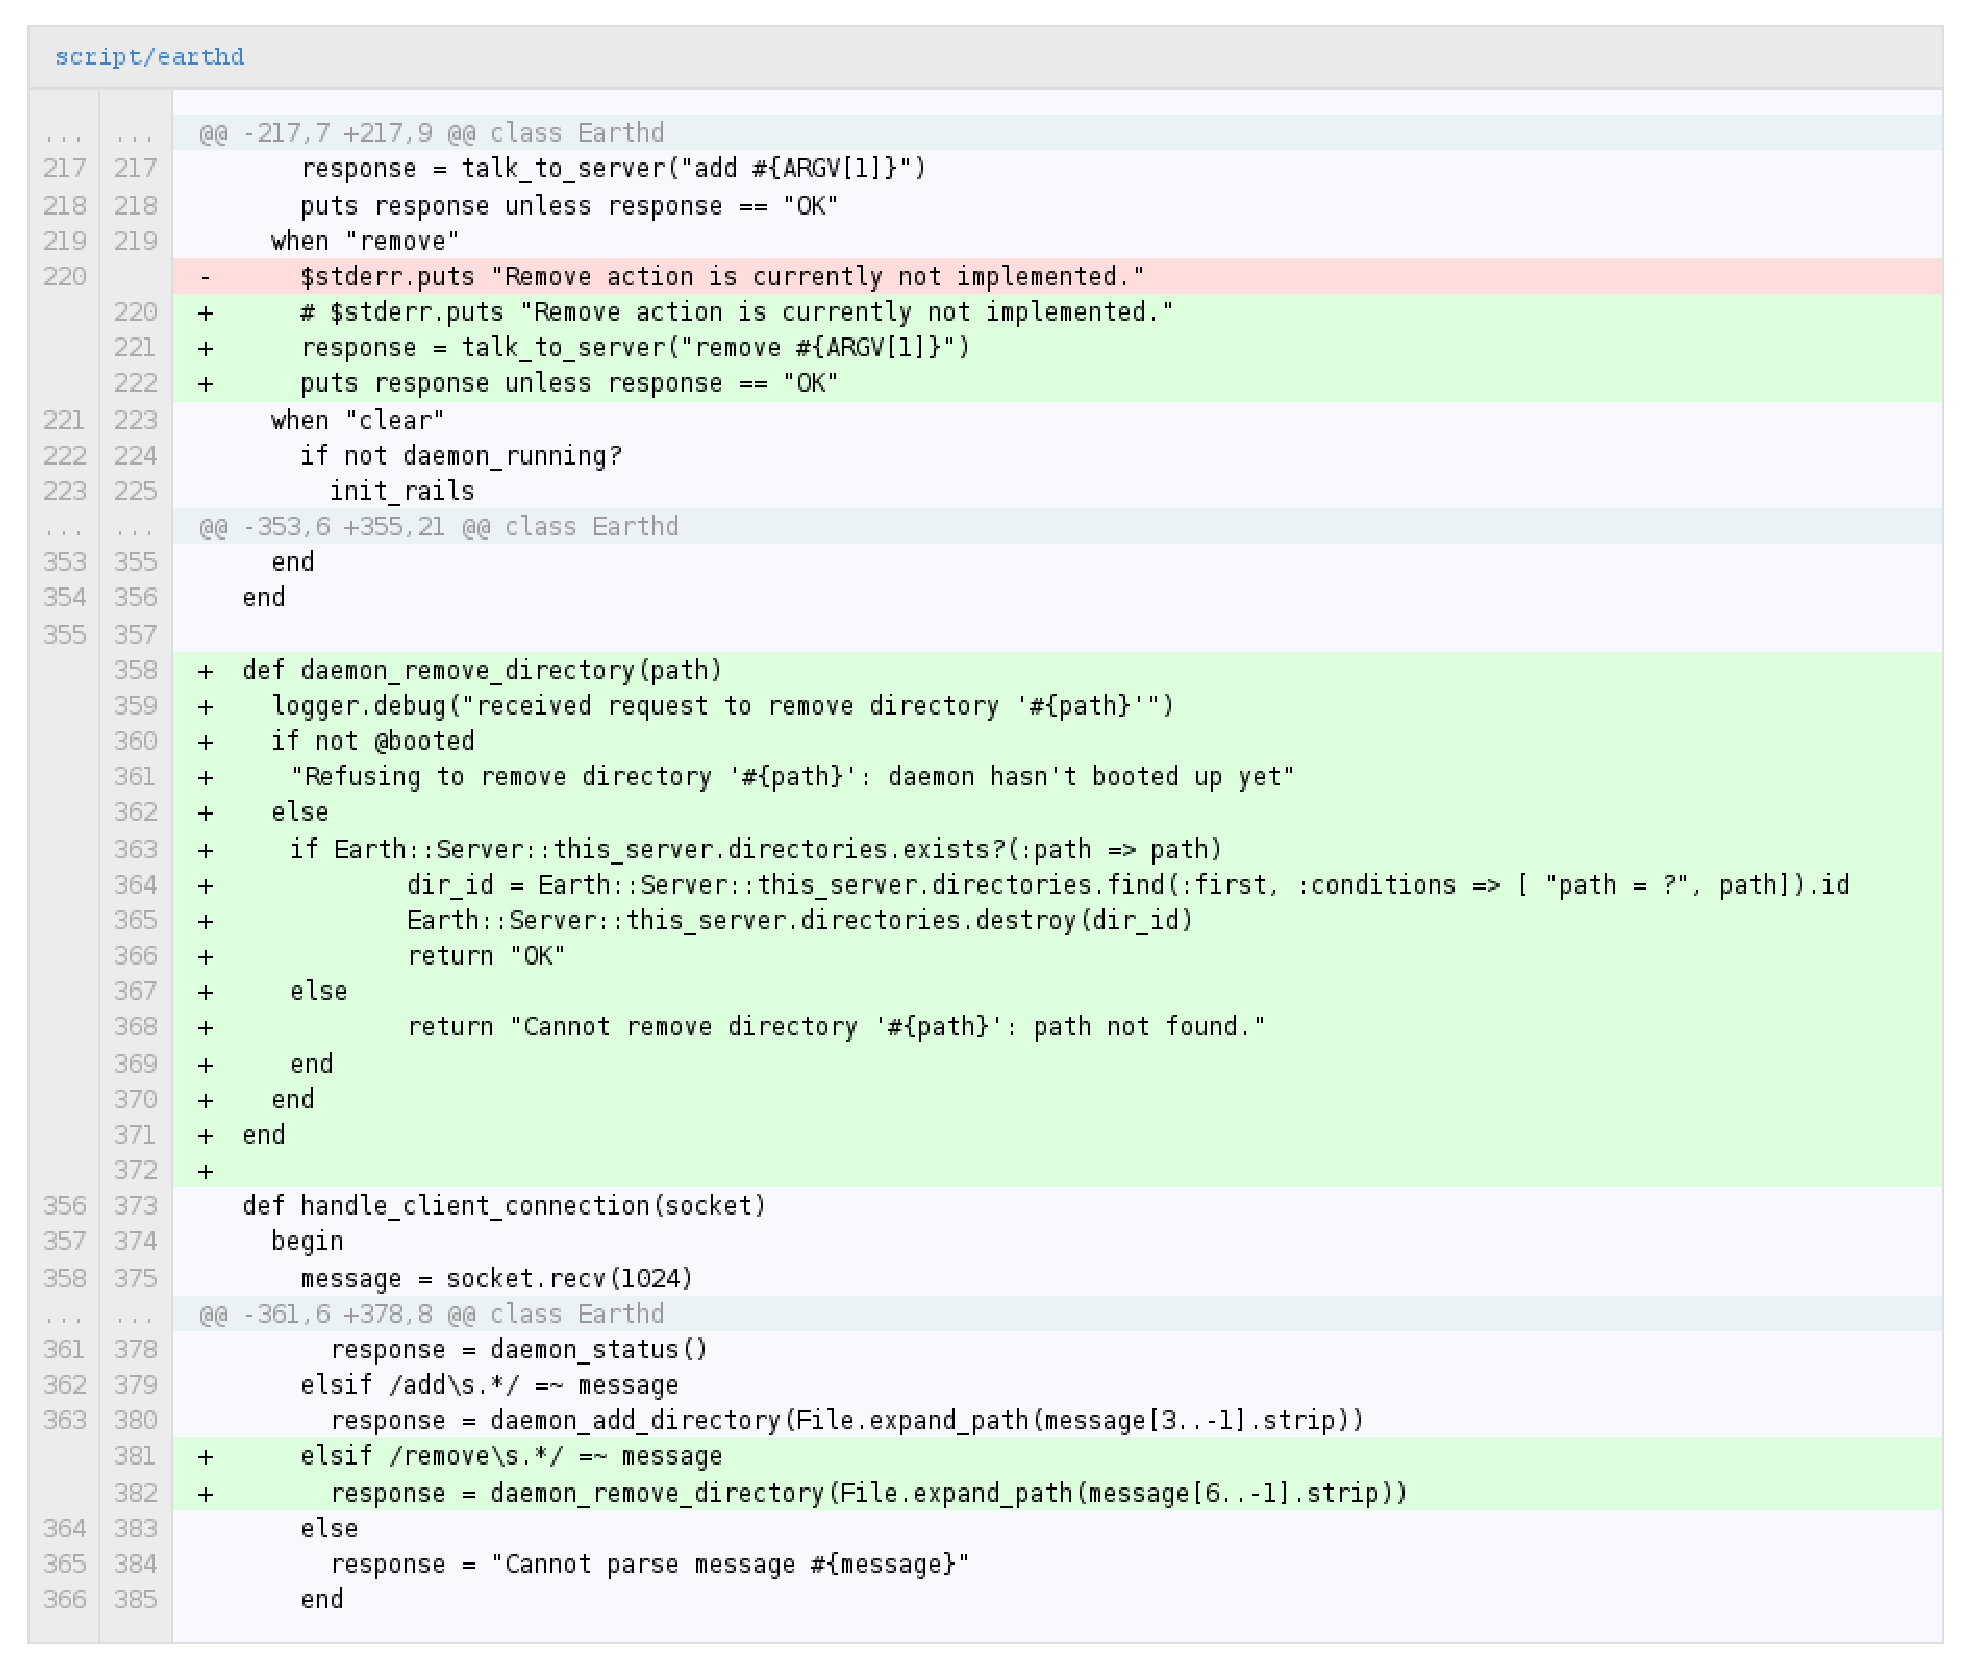
\includegraphics[width=150mm]{figs/earthd}
\end{centering}
\caption{Daemon code modification.}
\label{fig:earthd}
\end{figure}


\paragraph{Note:}
The added code snippets are highlighted green while the removed code 
snippets are highlighted red.


\newpage

\paragraph{}
Further modifications were then made to the code to ensure that the given 
path name is a valid directory as shown below.

\begin{figure}[h!]
\begin{centering}
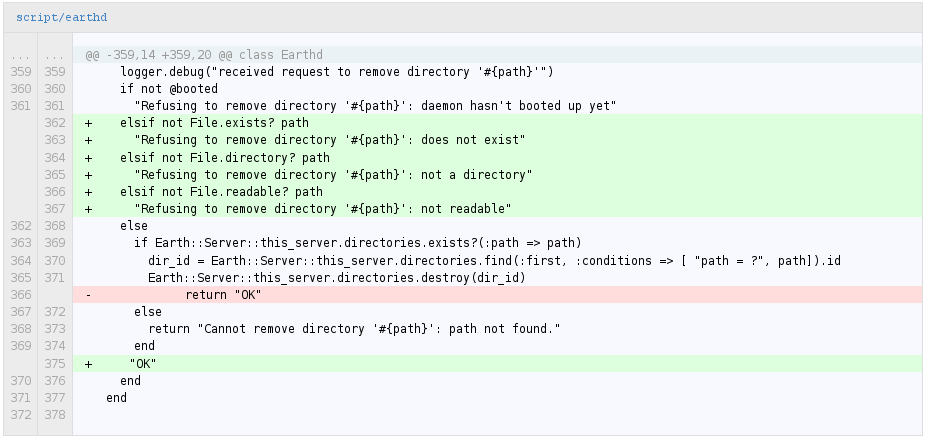
\includegraphics[width=150mm]{figs/earthd2}
\end{centering}
\caption{Validating directory path.}
\label{fig:earthd2}
\end{figure}


\newpage

\paragraph{}
The following changes were then made to the model, controller and view 
codes respectively to enable the execution of the directory removal 
feature from the web-based user interface.


\begin{figure}[h!]
\begin{centering}
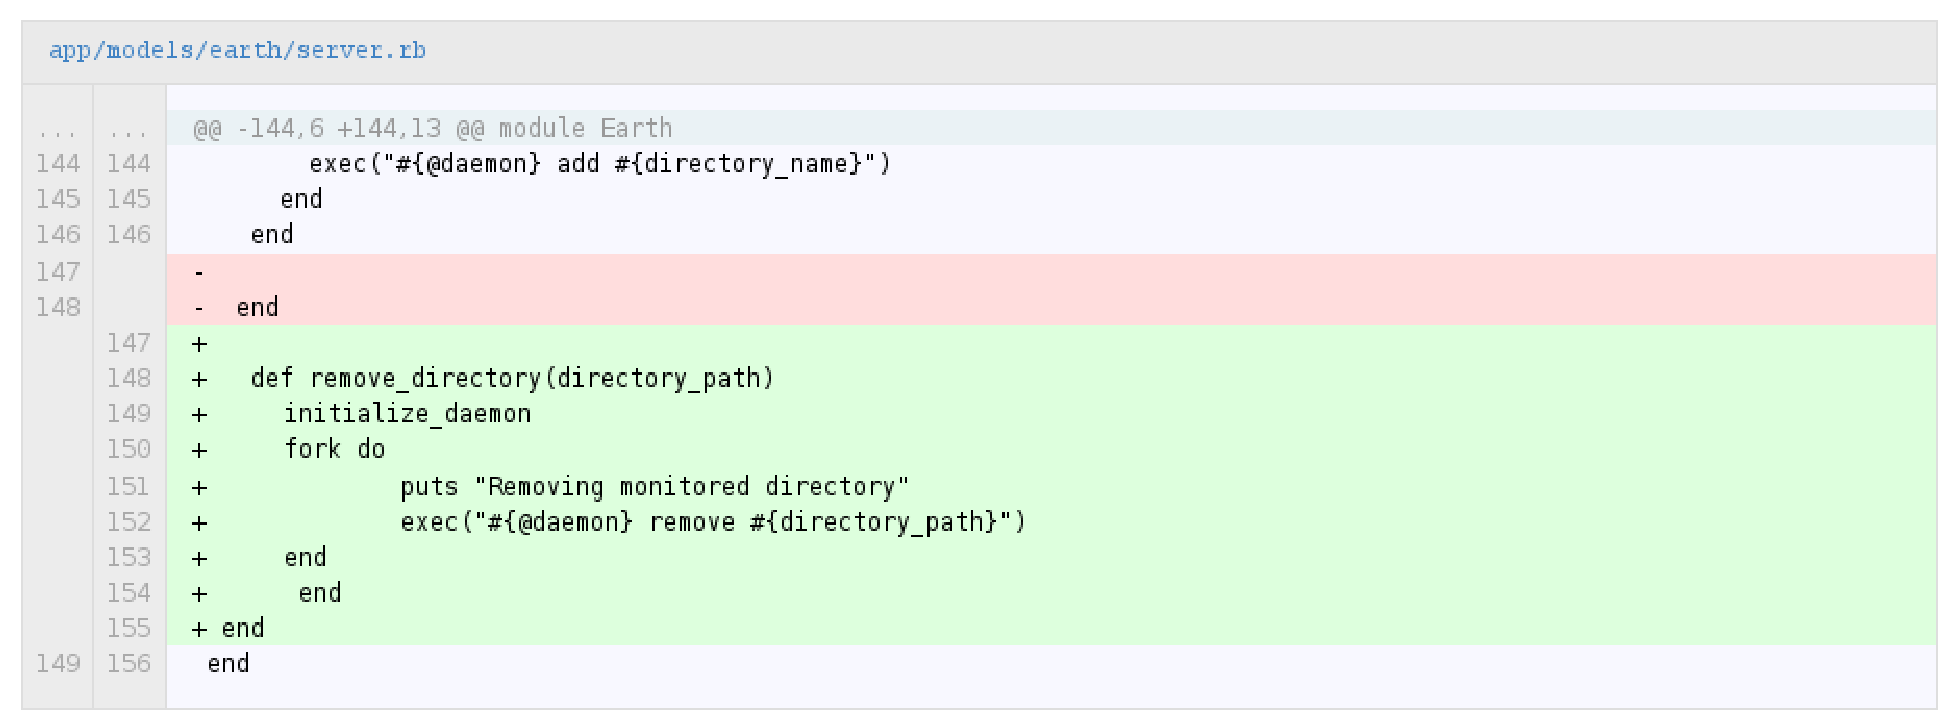
\includegraphics[width=150mm]{figs/earthmodel}
\end{centering}
\caption{Modified model code.}
\label{fig:earthmodel}
\end{figure}


\begin{figure}[h!]
\begin{centering}
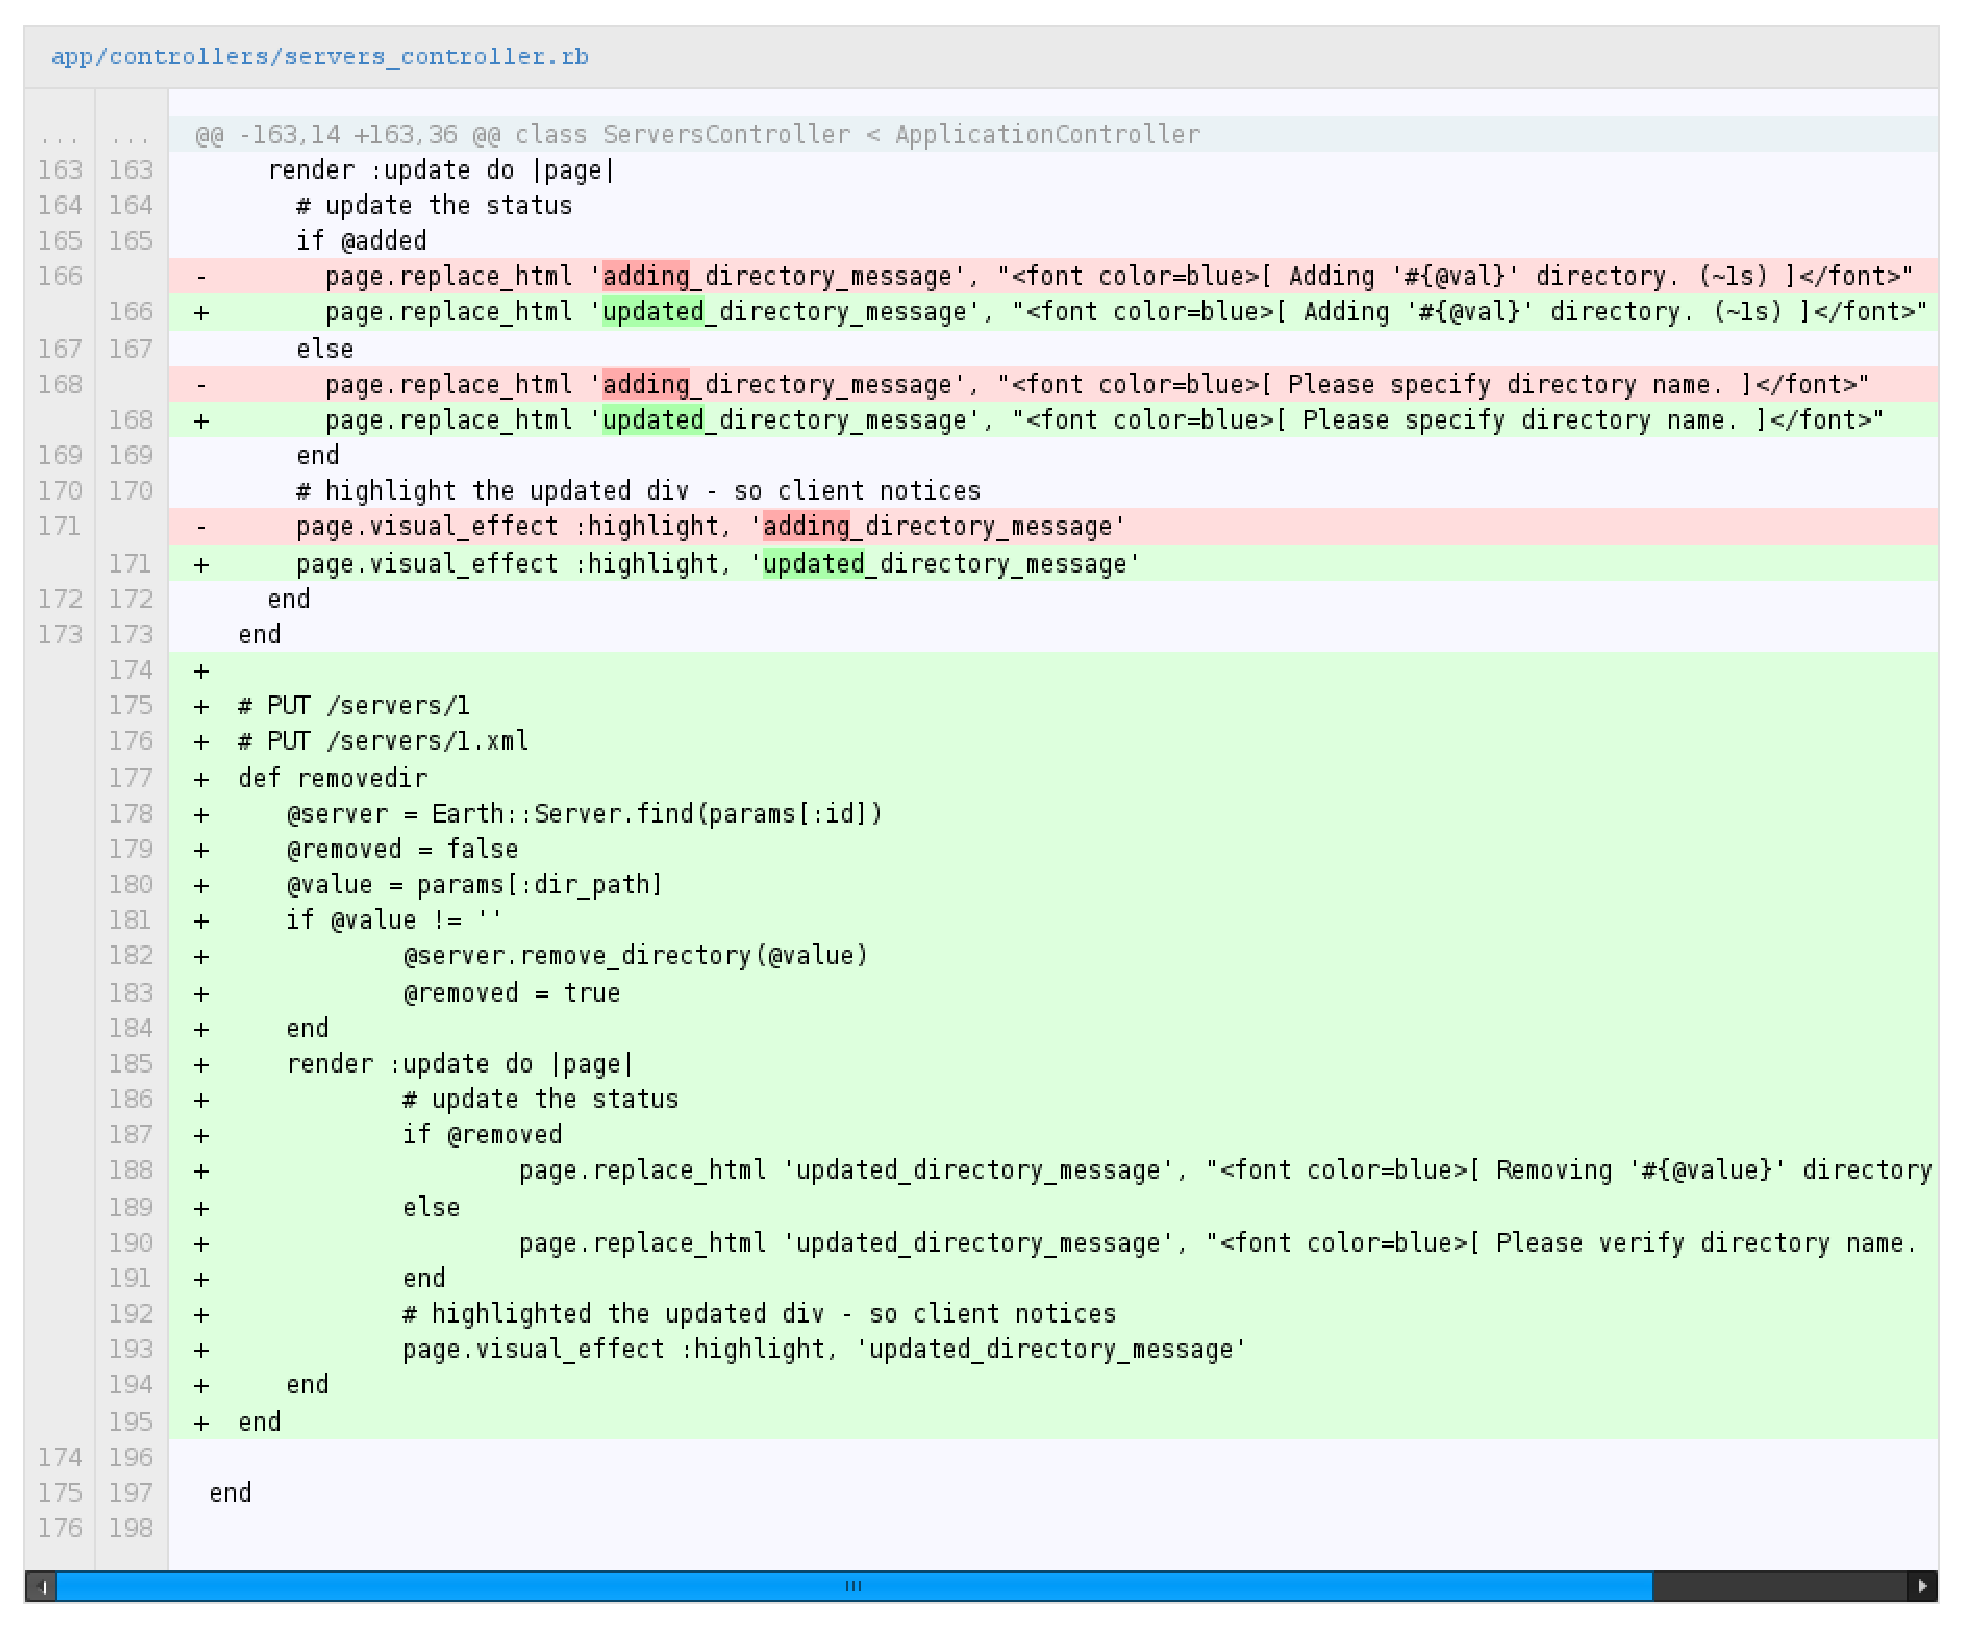
\includegraphics[width=150mm]{figs/earthcontroller}
\end{centering}
\caption{Modified controller code.}
\label{fig:earthcontroller}
\end{figure}


\begin{figure}[h!]
\begin{centering}
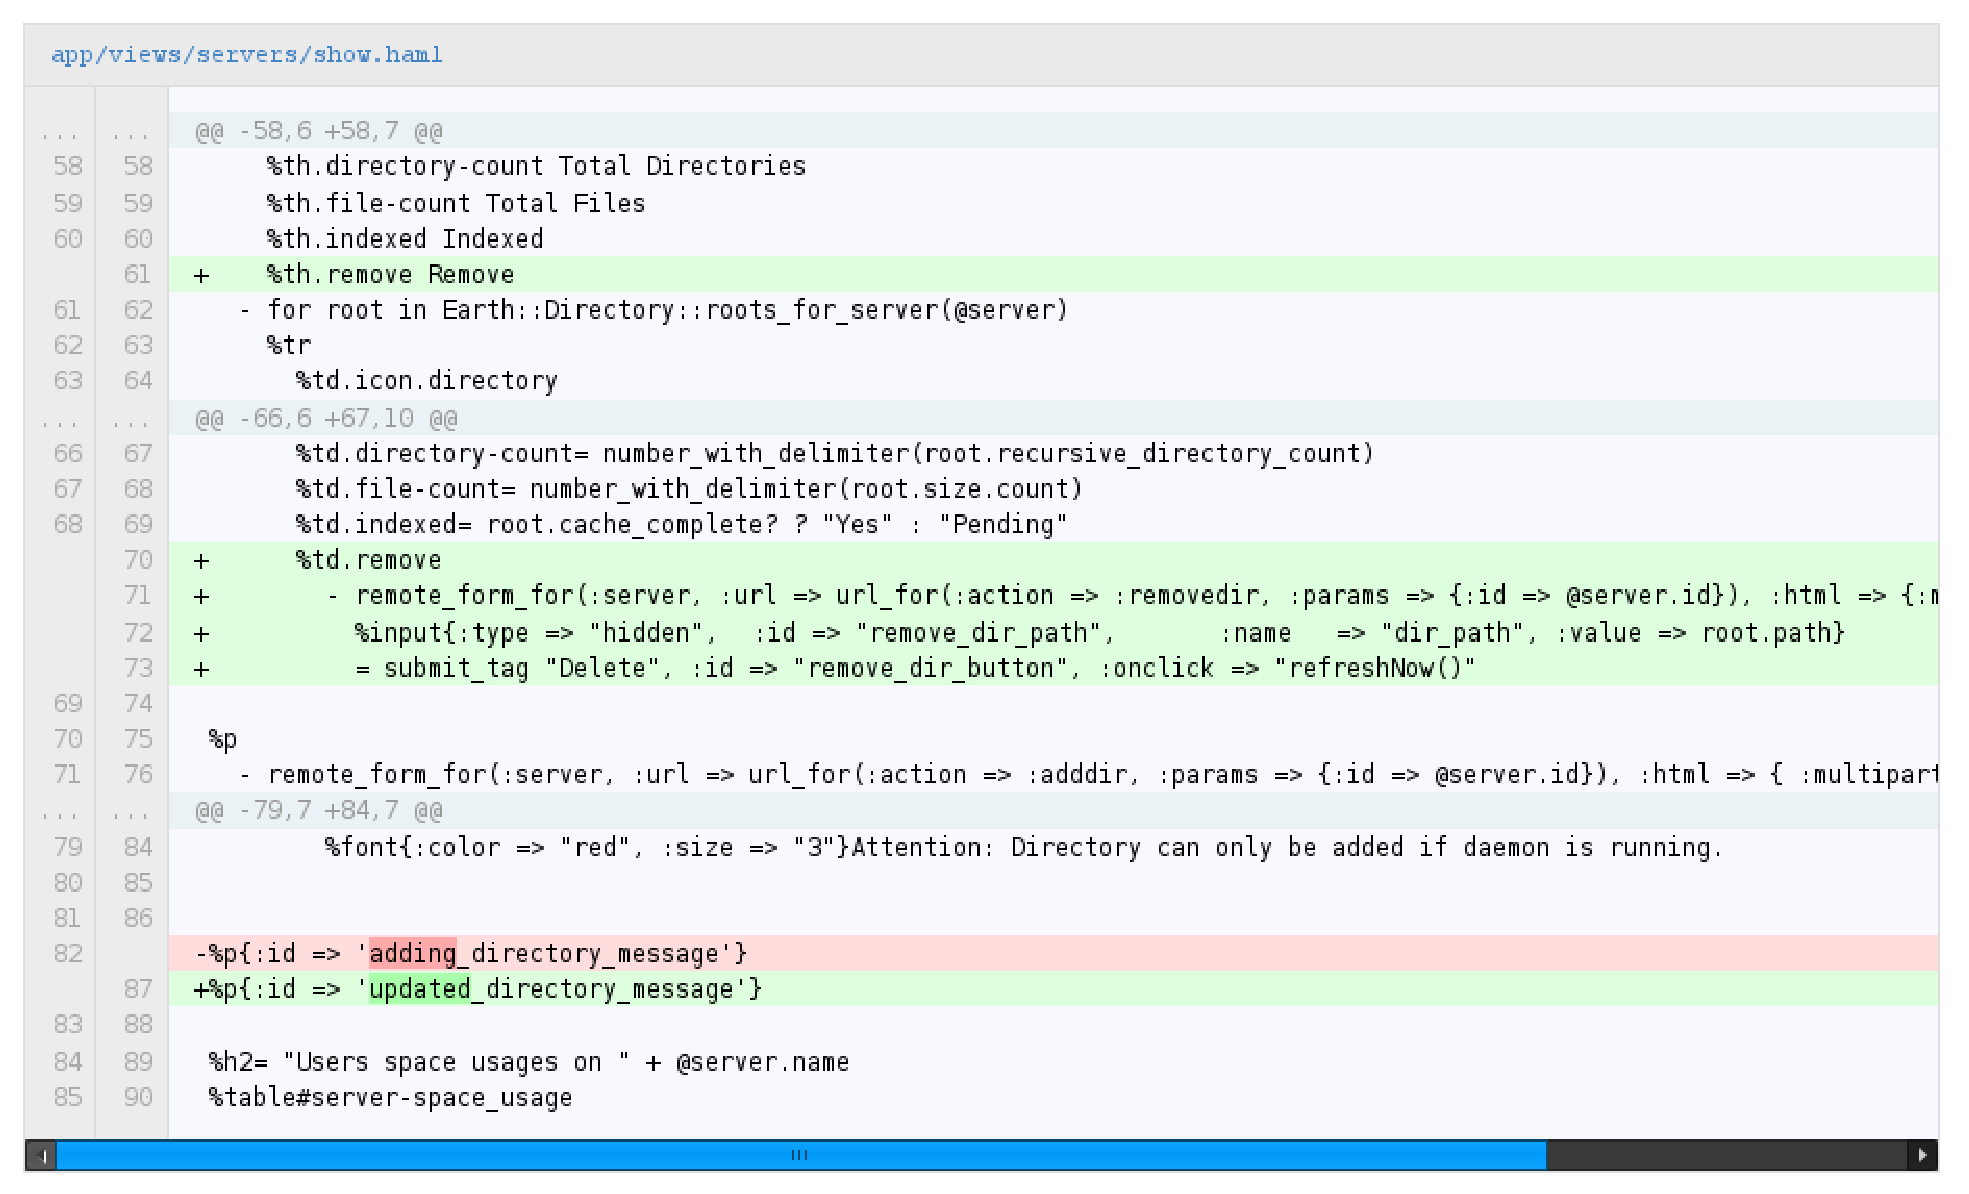
\includegraphics[width=150mm]{figs/earthview}
\end{centering}
\caption{Modified view code.}
\label{fig:earthview}
\end{figure}



\newpage

\paragraph{}
The following additional modification was then made to the view code 
to sort the list of monitored folder in ascending alphabetical order.


\begin{figure}[h!]
\begin{centering}
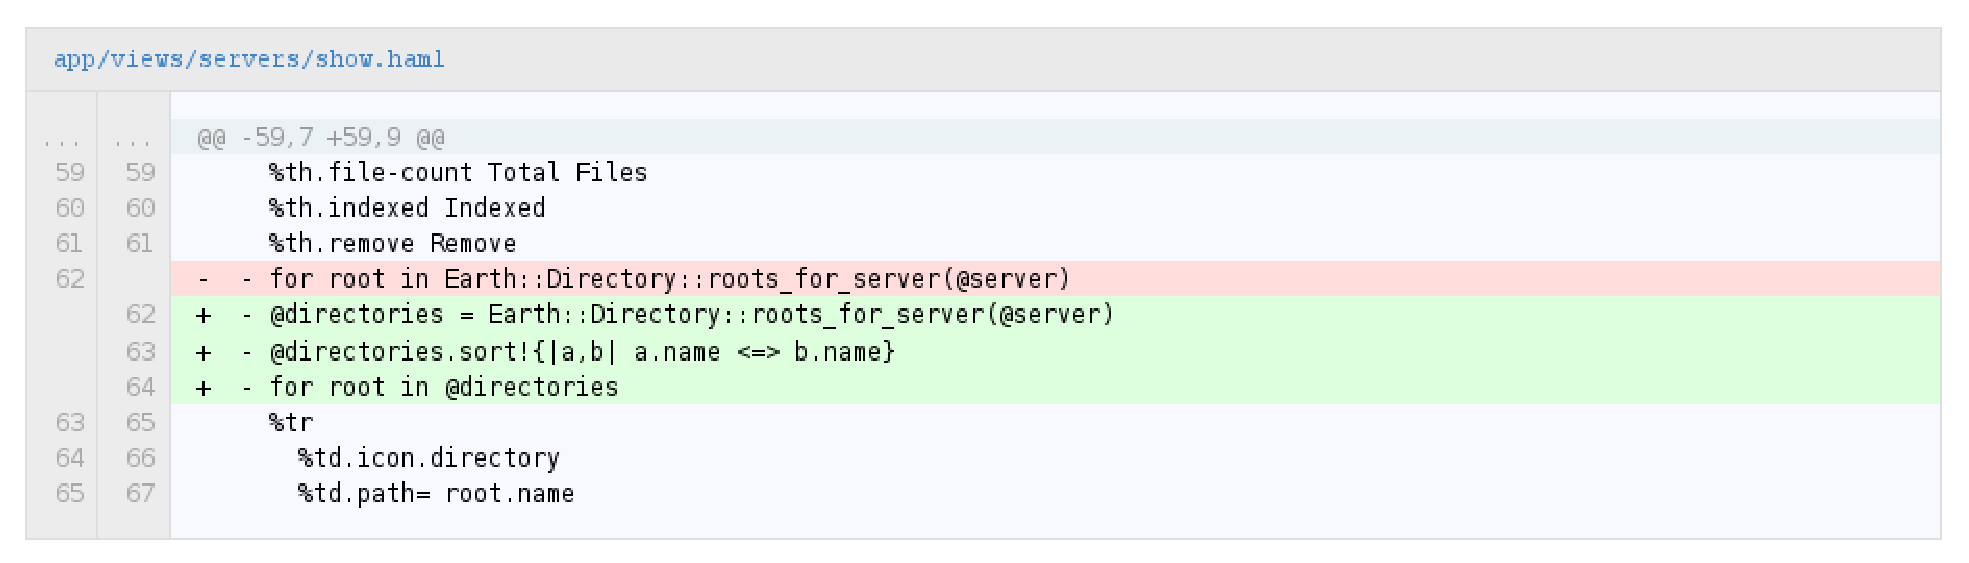
\includegraphics[width=150mm]{figs/earthshow2}
\end{centering}
\caption{Modified view code to sort directory listing.}
\label{fig:earthshow2}
\end{figure}


\newpage

\paragraph{}
Unfortunately, these changes would cause the unexpected termination 
of the daemon whenever the remove method is invoked. Apparently, the 
removal action introduced some inconsistencies between the cached 
data and the directories array which would trap the daemon on 
subsequent updates. The following modification was then made to the 
file monitor plugin to resolve this data consistency issue.



\begin{figure}[h!]
\begin{centering}
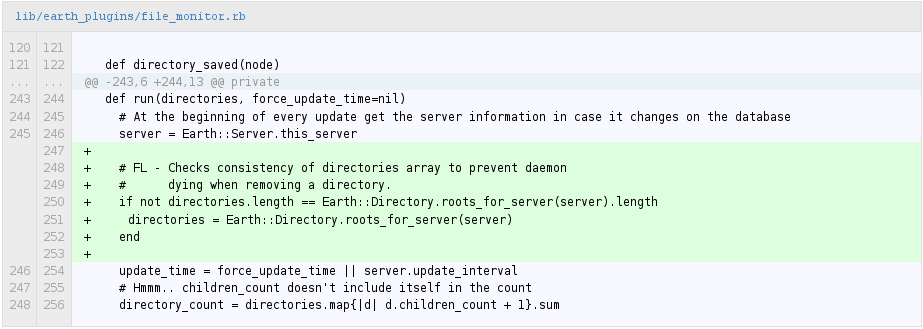
\includegraphics[width=150mm]{figs/filemonitor}
\end{centering}
\caption{Modified file monitor code to resolve data inconsistency.}
\label{fig:filemonitor}
\end{figure}


\paragraph{}
These changes effectively enabled the resulting implementation of 
the daemon remove feature. Further, these code modifications were 
pushed onto the remote github repository (ssurfer/earth.git) before 
it would be further propagated onto the Group 1 repository 
(segp2sg1/earth.git).



\newpage

\subsection*{Results}

\paragraph{}
Apart from the code snippets presented in the previous section, 
the only other visual outcome of this task were the delete buttons 
column on the monitored directories listing as shown in the 
following screenshot.


\begin{figure}[h!]
\begin{center}
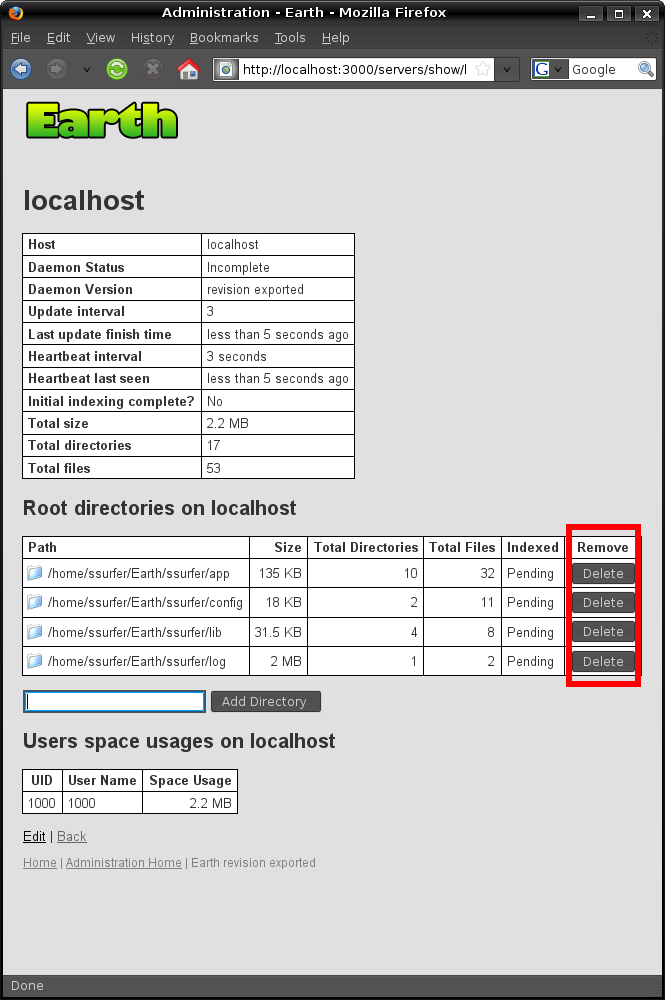
\includegraphics[width=90mm]{figs/screendel}
\end{center}
\caption{Directory listing with delete column.}
\label{fig:screendel}
\end{figure}


\newpage

\subsection*{Discussion}

\paragraph{}
For this task, the allocated time of 81 hours was adopted based 
on the feedback from Milestone 3 wherein a preliminary study was 
conducted. This time was subdivided into the following subtasks in 
the Milestone 4 Plan document:

\begin{enumerate}
\item Investigate the existing add feature of the daemon. (8hrs)
\item Identify the relevant components of the remove feature. (16hrs)
\item Design and code an effective implementation of the remove feature. (40hrs)
\item Test and integrate solution to the Subgroup 1 codebase. (16hrs)
\item Update the Earth Trac system. (1hr)
\end{enumerate}

\paragraph{}
The actual recorded work took 87 hours (log included as Appendix) which in 
hindsight, appeared to have been over budgeted for a relatively minor and 
isolated task. However, the task assumed an intermediate level of Ruby On Rails 
understanding and in-depth knowledge of the earth application. 
This particular skillset was limited at the commencement of this current 
milestone and a significant amount of resources (time) had to be expanded 
in order to complete the planned task. Nevertheless, a significant 
understanding of the earth application was attained as a result which 
would certainly be valuable for proceeding with the more challenging 
tasks of later milestones.

\paragraph{}

\subsection*{Conclusion}

\paragraph{}
The daemon remove feature was implemented with appropriate modifications 
in relevant files on the Earth project codebase. Further, a simple 
adaptation of the remove feature on the web user interface was included 
for completeness.

\paragraph{}

\subsection*{Acknowledgement}


\paragraph{}
The code snippets included in this document were extracted using the 
source view feature of the github repositories where the project 
codebase is controlled and distributed.

\paragraph{}


\newpage

\subsection*{Appendix - Development Log}

\paragraph{Note}
Figures rounded to nearest hour in some cases and every effort made 
to keep this log as accurate and informative as possible.

\begin{mylisting}
\begin{verbatim}

Semester 2 Week 1


Monday Jul 28, 2008

1300 - 1500 hrs

Attended main group meeting and discussed planned tasks for Milestone 4.

Daily Total: 2 hrs


Tuesday Jul 29, 2008

0800 - 1100 hrs

Drafted Milestone 4 plan for Group 1 and discussed resource planning with other group members.

1500 - 1700 hrs

Completed and submitted Milestone 4 plan for Group 1.

Daily Total: 5hrs


Wednesday Jul 30, 2008

0800 - 1100 hrs

Investigate implementation of add directory feature.

1300 - 1600 hrs

Revisit rails documentation on ActiveRecord::Base class. (Ref: The Rails Way)

1900 - 2100 hrs

Trace add directory implementation code through the application.

Daily Total: 8 hrs


Thursday Jul 31, 2008

0800 - 1100 hrs

Advanced Rails Tutorial (Ref: Wrox Beginning Rails).

1230 - 1530 hrs

Continued with Advanced Rails Tutorial (Ref: Wrox Beginning Rails).

Daily Total: 6 hrs


Friday Aug 1, 2008

0800 - 1100 hrs

Continued with Advanced Rails Tutorial (Ref: Wrox Beginning Rails).

1300 - 1600 hrs

Revisited earth code on add directory feature and identified remove feature components on MVC framework.

Daily Total: 6 hrs


Weekly Total:  27 hrs
========================================================================




Semester 2 Week 2


Monday Aug 4, 2008

1300 - 1400 hrs

Attended main group meeting and discussed progress.

1600 - 1900 hrs

Continued with coding as planned design had to revised.

Daily Total: 4 hrs


Tuesday Aug 5, 2008

1300 - 1600 hrs

Code and progressively test the remove feature implementation.

1800 - 2100 hrs

Continued with coding.

Daily Total: 6 hrs


Wednesday Aug 6, 2008

1400 - 1500 hrs

Attended Group 1 subgroup meeting with Dr. Li.

1800 - 2100 hrs

Continued with the coding. Delete method still doesn't work.

Daily Total: 4 hrs


Thursday Aug 7, 2008

0800 - 1100 hrs

Continued with coding.Monday Aug 3, 2008

1900 - 2200 hrs

Continued with coding.

Daily Total: 6 hrs


Friday Aug 8, 2008

1300 - 1600 hrs

Revisited base class to find out the SQL statement of the delete and delete_all method.

1800 - 2200 hrs

Still no luck with actual removal action.

Daily Total: 6 hrs


Weekly Total:  26 hrs
========================================================================









Semester 2 Week 3

Sunday Aug 10, 2008

1000 - 1400 hrs

Tested various methods in ActiveRecord::Base class to identify most suitable removal method.

1600 - 1800 hrs

Identified the 'destroy' class method in ActiveRecord::Base as the best option to remove directory 
for the daemon.

Daily Total: 6 hrs


Monday Aug 11, 2008

1300 - 1400 hrs

Group Meeting at SE Meeting Room

2000 - 0000hrs

Investigated the termination of the daemon when removing a directory. Still not resolved.

Daily Total: 5 hrs


Tuesday Aug 12, 2008

1200 - 1530 hrs

Traced through daemon execution sequence to identify termination condition.

1700 - 2330 hrs

Continued with above unresolved task.

Daily Total: 10 hrs


Wednesday Aug 13, 2008

1000 - 1500 hrs

Devised test script to trap daemon execution sequence. Found 'culprit' code in file monitor 
plugin module (file_monitor.rb).

Daily Total: 5 hrs


Thursday Aug 14, 2008

2000 - 2300 hrs

Verified conformance of remove feature with existing unit tests.

Daily Total: 3 hrs


Friday Aug 15, 2008

0800 - 1000 hrs

Repeated unit and function tests. Updated remote group 1 repository (segp2sg1/earth.git).

1130 - 1330 hrs

Tested repository code on uni machine and prepared for group presentation.

1400 - 1500 hrs

Attended milestone 4 presentation.

Daily Total: 5 hrs


Weekly Total: 34 hrs
========================================================================


\end{verbatim}
\end{mylisting}

\[----\]

\newpage

\section{Individual Milestone 4 Report - George Leonard Sainsbury}

\subsection*{Progress Report}

\paragraph{}
At the end of Milestone 4, this ticket is completed, though it raises more issues. On the surface, creating a gem is very easy. The gem specification file has been completed and the gem can successfully be packaged and installed. What remains is to ascertain the usefulness of this ticket. There seems to be little or no immediate benefit in earth being packaged into a gem in this way. These questions will be raised at the upcoming meeting with RSP and  hopefully addressed and answered then.

\subsection*{Time Log}
\begin{itemize}
 \item Assessing progress from previous milestone: 1 hour.
 \item Addressing the problem of files not being placed inside the  
gem and working out a solution: 2 hours.
 \item Successfully creating and installing a gem and verifying its  
contents: 2 hours.
 \item Investigation of signing process: 1 hour.
\end{itemize}

\newpage

\section{References}

Earth Project, \textit{Ticket 75} Retrieved from \emph{http://open.rsp.com.au/projects/earth/ticket/75} \\
\newline
Earth Project, \textit{Ticket 131} Retrieved from \emph{http://open.rsp.com.au/projects/earth/ticket/131} \\
\newline
Earth Project, \textit{Ticket 186} Retrieved from \emph{http://open.rsp.com.au/projects/earth/ticket/186} \\
\newline
Earth Project, \textit{Ticket 174} Retrieved from \emph{http://open.rsp.com.au/projects/earth/ticket/174} \\

\paragraph{}

\[\emph{End}\]
\end{document}